\documentclass[11pt,letterpaper]{article}

\usepackage[margin=1in]{geometry}
\usepackage{amsmath, amssymb, amsthm}
\usepackage{graphicx}
\usepackage{tikz}
\usetikzlibrary{positioning, shapes.geometric, arrows.meta, fit, backgrounds, calc}
\usepackage{booktabs}
\usepackage{xcolor}
\usepackage{colortbl}
\usepackage{hyperref}
\usepackage{caption}
\usepackage{enumitem}
\usepackage{microtype}
\usepackage{array}

% Loosen line-breaking on paragraphs with long compound words
\emergencystretch=3em
\hyphenation{roof-line-derived reasoning-versus-chat throughput-oriented deadline-aware admission-control cross-comparison per-tenant per-request per-stage}

% Palette used ONLY for diagram fills / table row shading (not text)
\definecolor{admitteal}{HTML}{1E7882}
\definecolor{admitteallight}{HTML}{D1E7EA}
\definecolor{admityellow}{HTML}{F0C83C}
\definecolor{admityellowlight}{HTML}{FBEFC8}
\definecolor{admitgrey}{HTML}{808080}
\definecolor{admitgreylight}{HTML}{E5E5E5}

% All text black. Hyperlinks black (readable in print).
\hypersetup{
  colorlinks=true,
  linkcolor=black,
  citecolor=black,
  urlcolor=black,
  linktoc=all
}

\begin{document}

\begin{center}
{\LARGE\bfseries Admission Control for LLM Inference Serving:\\[0.2em] A Systematic Review\par}

\vspace{1em}
{\color{admitgrey}\rule{0.55\textwidth}{0.6pt}}
\vspace{1em}

{\normalsize
\renewcommand{\arraystretch}{1.15}
\begin{tabular}{ccc}
\textbf{Harshul Jain} & \textbf{Dr.\ Tanmay Sah} & \textbf{Tanya Sah} \\
Independent Researcher & Independent Researcher & Independent Researcher \\
{\small\texttt{harshuljain1393@gmail.com}} & {\small\texttt{tradertanmay@mail.com}} & {\small\texttt{tanyasah20@gmail.com}} \\
\end{tabular}
}

\vspace{0.8em}
{\itshape September 11, 2026}
\end{center}

\vspace{1em}

\begin{abstract}
\noindent
Serving large language models at scale is a distributed systems problem
whose overload behavior is governed at the ingress. Yet an audit of nine
top-venue scheduling papers from OSDI, SOSP, ASPLOS, EuroSys, MLSys, and
HPCA between 2022 and 2026 finds that not one includes an explicit
ingress-level admission control policy. All nine respond to overload
through batching, migration, placement, autoscaling, or memory
management. In parallel, thirteen peer-reviewed papers at top venues
plus one accepted workshop paper and more than a dozen preprints
propose admission policies operating at request, agent-session, or
tenant granularity, under online or offline settings, guided by cache
pressure, deadline slack, queue depth, or joint linear programs. No two
of these policies have been compared to each other on a common trace,
engine, or metric. We survey forty admission and admission-adjacent
works. We propose a four-axis taxonomy with sub-branches for signal
structure, service-level-objective granularity, fairness type, and
concurrency context. The canonical intersection agent-level $\times$
online $\times$ deadline-aware $\times$ fair is empty. We audit
reproducibility across the corpus and find that thirteen of thirty-four
works have released code, refuting the common ``reproducibility
crisis'' framing at the artifact level, while a methodology-level
crisis persists because no two admission-primary papers share a
baseline set. We propose a minimal common methodology contract to close
that gap. We derive seven open problems, each grounded in either
published peer-review discussion or the primary source's own limitation
statement.
\end{abstract}

\section{Introduction}

On November 8, 2023, OpenAI's inference fleet crossed a soak point after
a day of unusually heavy completion traffic. Routing nodes reached
memory limits and failed readiness checks. Additional replicas were
added, then rolled back. Recovery required cutting inbound traffic,
redeploying, and slowly ramping load back up. The postmortem named
graceful load shedding through stronger rate-limit controls as the
required follow-up. Two years later, on January 21, 2026, Anthropic's
Sonnet 4.5 tier degraded first in latency and then in error rate over
roughly ninety minutes. The postmortem cited insufficient compute
capacity for demand and named earlier detection of capacity constraints
as a required change. Cloudflare, Azure, and other production operators
have documented similar sequences.

Admission control is the decision made before a request enters the
running batch. It has three actions: admit into service, hold in queue,
or reject with a well-defined error contract. Figure~\ref{fig:aqr}
depicts the model. When admission is wrong, downstream batching, KV
cache management, and preemption cannot recover lost capacity. Requests
admitted past a soak point occupy memory until they miss their
deadline, at which point they consume more capacity being cleaned up.

\begin{figure}[htbp]
\centering
\resizebox{0.95\textwidth}{!}{%
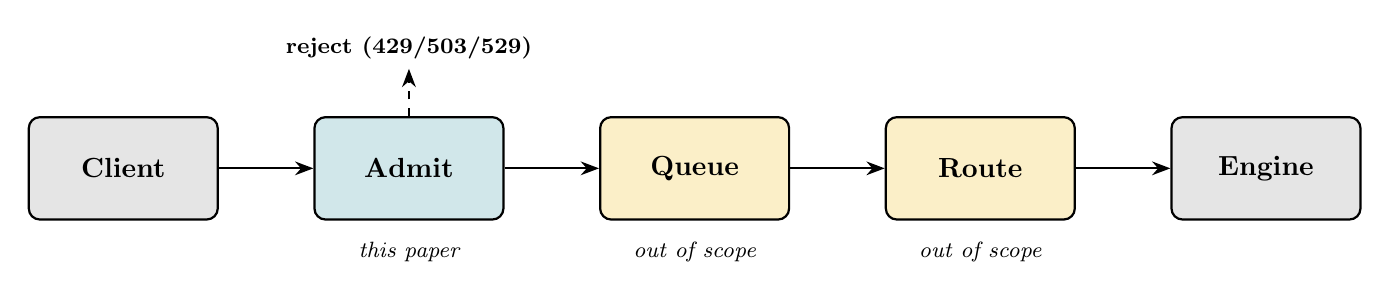
\begin{tikzpicture}[
  node distance=1.2cm and 1.2cm,
  box/.style={rectangle, rounded corners, minimum width=2.4cm, minimum height=1.3cm, text centered, draw=black, thick, font=\bfseries, fill=admitteallight},
  ybox/.style={rectangle, rounded corners, minimum width=2.4cm, minimum height=1.3cm, text centered, draw=black, thick, font=\bfseries, fill=admityellowlight},
  gbox/.style={rectangle, rounded corners, minimum width=2.4cm, minimum height=1.3cm, text centered, draw=black, thick, font=\bfseries, fill=admitgreylight},
  arr/.style={-Stealth, thick, black},
  label/.style={font=\footnotesize\itshape, black}
]

\node[gbox] (client) {Client};
\node[box, right=of client] (admit) {Admit};
\node[ybox, right=of admit] (queue) {Queue};
\node[ybox, right=of queue] (route) {Route};
\node[gbox, right=of route] (engine) {Engine};

\draw[arr] (client) -- (admit);
\draw[arr] (admit) -- (queue);
\draw[arr] (queue) -- (route);
\draw[arr] (route) -- (engine);

\node[below=0.15cm of admit, label] {this paper};
\node[below=0.15cm of queue, label] {out of scope};
\node[below=0.15cm of route, label] {out of scope};

\node[above=0.6cm of admit, font=\footnotesize\bfseries] (rej) {reject (429/503/529)};
\draw[arr, dashed] (admit.north) -- (rej.south);

\end{tikzpicture}%
}
\caption{The Admit--Queue--Route model. Admission is the decision that gates a request into the serving pipeline. Queue and Route are downstream boxes covered by prior surveys. This paper is about the first box.}
\label{fig:aqr}
\end{figure}

The literature on LLM inference has produced systems papers on batching
\cite{yu2022orca, agrawal2024sarathi}, disaggregation
\cite{zhong2024distserve, patel2024splitwise}, memory management
\cite{kwon2023pagedattention, qin2025mooncake}, and scheduling
\cite{sun2024llumnix, hong2025sola}. Existing surveys cover efficient
serving broadly \cite{zhen2025titans, li2024surveyllm,
heisler2025survey} or the queueing-theoretic view of LLM systems
specifically \cite{mitzenmacher2025queueing}. Table~\ref{tab:diff}
differentiates this survey from those prior works.

\paragraph{Contributions.}
\begin{enumerate}[leftmargin=1.5em, itemsep=2pt]
\item A four-axis taxonomy for admission-control policies with four
      sub-branches added during the reading (Section~\ref{sec:taxonomy}).
\item A per-cluster synthesis of forty admission and admission-adjacent
      works (Section~\ref{sec:clusters}).
\item An empirical reproducibility audit across the corpus
      (Section~\ref{sec:repro}), showing thirteen of thirty-four works
      have released code and that the real crisis is methodological.
\item A proposed minimal common methodology contract that would enable
      cross-paper comparison without demanding that any paper change
      its primary evaluation (Section~\ref{sec:repro}).
\item A mapping of production incidents to admission failure modes
      (Section~\ref{sec:prod}).
\item Seven open problems, each with cited evidence from either public
      peer review or the primary source's own limitations
      (Section~\ref{sec:open}).
\end{enumerate}

\paragraph{Headline observations.} First, of nine top-venue scheduling
papers we audited, none includes an ingress-level admission policy;
overload is absorbed by batching, migration, placement, autoscaling, or
memory management. Second, of fourteen admission-primary papers we
audited, no two share a baseline system, metric definition, trace,
model, or engine. Third, the taxonomy holds across all forty works with
four sub-branches added during our reading, none of which required
backing out an original axis.

\paragraph{Roadmap.} Section~\ref{sec:bg} covers the inference request
lifecycle and the Admit-Queue-Route model.
Section~\ref{sec:taxonomy} introduces the four-axis taxonomy.
Section~\ref{sec:method} describes the systematic-review method.
Section~\ref{sec:clusters} synthesizes each policy cluster.
Section~\ref{sec:repro} audits reproducibility and proposes the
methodology contract. Section~\ref{sec:prod} maps production incidents
to admission failure modes. Section~\ref{sec:open} lists the seven
open problems. Section~\ref{sec:conc} concludes.

\subsection{Related surveys and differentiation}

Four broad surveys of LLM inference serving predate this work.
Table~\ref{tab:diff} summarizes each and states what this paper adds.

\begin{table}[htbp]
\centering
\caption{Differentiation from prior surveys.}
\label{tab:diff}
\small
\rowcolors{2}{white}{admitgreylight!40}
\begin{tabular}{p{3.4cm} p{3.2cm} p{2.2cm} p{2.4cm} p{2cm}}
\toprule
\rowcolor{admitteallight}
\textbf{Prior survey} & \textbf{Scope} & \textbf{Admission depth} & \textbf{Taxonomy axes} & \textbf{Grounded open problems} \\
\midrule
Zhen et al.\ INLG 2025 & Efficient serving (batching, KV, sched., fair.) & One subsection & Task-oriented & No \\
Heisler et al.\ TechRxiv 2025 & Scheduling techniques \& trade-offs & Component & Technique-oriented & No \\
Li et al.\ IEEE HPEC 2024 & Recent serving advances & In passing & Chronological & No \\
Mitzenmacher \& Shahout SIGMETRICS 2025 & Queueing theory position paper & Tutorial & Queueing-theoretic & Enumerates 25 \\
\rowcolor{admitgreylight}
\textbf{This paper} & \textbf{Admission as primary axis} & \textbf{Full} & \textbf{4 axes + 4 sub-branches} & \textbf{7 grounded} \\
\bottomrule
\end{tabular}
\end{table}

Zhen et al.\ and Heisler et al.\ treat admission as one component among
many. Li et al.\ is a survey of recent advances organized
chronologically. Mitzenmacher and Shahout is a position paper that
enumerates open queueing problems without a taxonomy or per-paper
review. None conducts a reproducibility audit or organizes the
literature by admission granularity, SLO awareness, signal structure,
or concurrency context.

\section{Background}
\label{sec:bg}

\subsection{The inference request lifecycle}

A large language model inference request passes through prefill,
decode, and completion. Prefill computes the key-value tensors for
every input token. Decode generates output tokens one at a time,
reading the accumulated KV cache and appending a new pair per step.
Continuous batching \cite{yu2022orca} reuses a single GPU-resident
engine across many concurrent requests by interleaving iterations at
token granularity. PagedAttention \cite{kwon2023pagedattention} manages
the KV cache in fixed-size blocks to reduce fragmentation and enable
prefix sharing.

The KV cache is the memory hierarchy's dominant consumer. It grows
monotonically with generated tokens during a request's decode, and it
persists across turns for multi-turn agents. When aggregate KV
footprint approaches available GPU memory, the engine must either
evict (recompute later), swap (page to CPU or disk), or preempt (kill
the request and return an error).

\subsection{The Admit--Queue--Route model}

Every request that reaches an inference cluster passes through three
decision boxes before it produces its first token
(Figure~\ref{fig:aqr}). \textbf{Admit} decides whether to accept the
request into service. \textbf{Queue} decides in what order accepted
requests are served. \textbf{Route} decides which replica or instance
receives the request. This paper is about the first box.

The error contract matters. HTTP 429 signals a client-side rate limit
exceeded. HTTP 503 signals a temporarily unavailable service.
Anthropic uses HTTP 529 to signal a provider-overloaded state distinct
from either \cite{anthropic_api_errors}. A well-designed admission
policy chooses among these codes based on which signal the client's
backoff logic should trust.

\subsection{Service-level objectives}

The community reports admission behavior against a small set of
metrics. Time-to-first-token (TTFT) is the wall-clock delay between
arrival and the first generated token. Time-between-tokens (TBT),
sometimes called inter-token latency or time-per-output-token (TPOT),
is the delay between consecutive generated tokens. Goodput is the
completed-request rate that met their service-level objective, distinct
from raw throughput \cite{zhong2024distserve}. For agentic workloads,
agent-completion rate measures the fraction of multi-turn sessions
that finish within an end-to-end budget.

\subsection{Why admission control is hard}
\label{sec:whyhard}

Ao, Dong, Luo, and Simchi-Levi \cite{ao2026sic} formalize the core
problem. In a discrete-time model of continuous batching under a memory
budget, the service process itself creates future capacity pressure
because each active request's KV footprint grows with each generated
token. They prove that the natural eviction-free equilibrium is
unstable under any admission rule that only checks instantaneous
memory feasibility. Along the resulting limit cycle the throughput
ratio equals
%
\begin{equation}
\rho^{\ast} \;=\; \frac{2\ell_0 + \ell_1 + 1}{2(\ell_0 + \ell_1)}
\label{eq:throughput-bound}
\end{equation}
%
which lies in $(1/2, 1)$ and converges to $1/2$ as
$\ell_1/\ell_0 \to \infty$. Their Theorem~3 further shows that
stability depends on the greatest common divisor of active decoding
lengths: if $\gcd(\ell_{1,1}, \dots, \ell_{1,K}) = g > 1$, unstable
modes appear on $g$-th roots of unity and synchronize into eviction
cycles; if $g = 1$, all roots lie strictly inside the unit disc and
the eviction-free equilibrium is globally asymptotically stable. This
is a workload-arithmetic property of admission decisions that no
production system currently exposes as a signal.

\section{Taxonomy}
\label{sec:taxonomy}

We organize admission-control policies along four axes.
Figure~\ref{fig:taxonomy} shows the two most-cited axes plotted
against each other with representative policies placed on the grid.

\begin{figure}[htbp]
\centering
\resizebox{0.9\textwidth}{!}{%
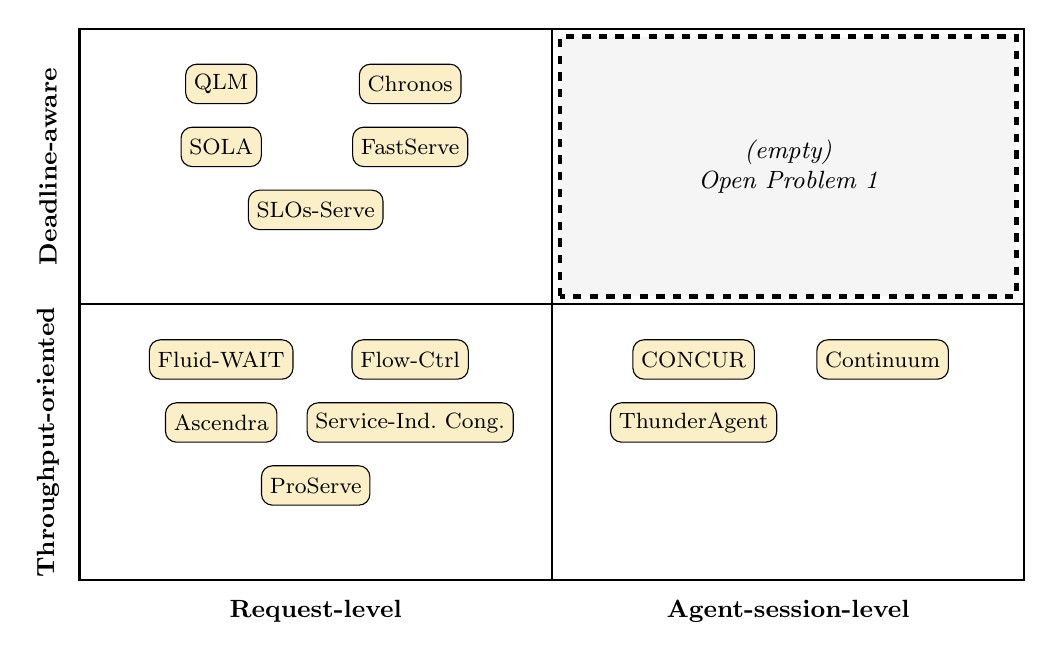
\begin{tikzpicture}[
  policy/.style={rectangle, rounded corners, minimum height=0.5cm, inner sep=3pt, fill=admityellowlight, draw=black, thin, font=\footnotesize},
  axislbl/.style={font=\bfseries\small},
  emptylbl/.style={font=\itshape\small, align=center}
]

% Frame
\draw[thick] (0, 0) rectangle (12, 7);
\draw[thick] (6, 0) -- (6, 7);
\draw[thick] (0, 3.5) -- (12, 3.5);

% Axis labels
\node[axislbl] at (3, -0.4) {Request-level};
\node[axislbl] at (9, -0.4) {Agent-session-level};
\node[axislbl, rotate=90] at (-0.4, 1.75) {Throughput-oriented};
\node[axislbl, rotate=90] at (-0.4, 5.25) {Deadline-aware};

% Q1: request x throughput
\node[policy] at (1.8, 2.8) {Fluid-WAIT};
\node[policy] at (4.2, 2.8) {Flow-Ctrl};
\node[policy] at (1.8, 2.0) {Ascendra};
\node[policy] at (4.2, 2.0) {Service-Ind.\ Cong.};
\node[policy] at (3.0, 1.2) {ProServe};

% Q2: agent x throughput
\node[policy] at (7.8, 2.8) {CONCUR};
\node[policy] at (10.2, 2.8) {Continuum};
\node[policy] at (7.8, 2.0) {ThunderAgent};

% Q3: request x deadline
\node[policy] at (1.8, 6.3) {QLM};
\node[policy] at (4.2, 6.3) {Chronos};
\node[policy] at (1.8, 5.5) {SOLA};
\node[policy] at (4.2, 5.5) {FastServe};
\node[policy] at (3.0, 4.7) {SLOs-Serve};

% Q4: empty
\draw[dashed, ultra thick, fill=admitgreylight!40] (6.1, 3.6) rectangle (11.9, 6.9);
\node[emptylbl] at (9, 5.25) {(empty)\\ Open Problem 1};

\end{tikzpicture}%
}
\caption{Policy taxonomy on Unit of admission (horizontal) $\times$
SLO awareness (vertical). The upper-right quadrant (agent-session
$\times$ deadline-aware) is empty; no published policy sits in that
intersection. This is the seed for Open Problem~1.}
\label{fig:taxonomy}
\end{figure}

\subsection{Axis 1: Unit of admission}

Admission decisions can be made at three granularities. Request-level
policies admit or reject each incoming prompt independently (QLM
\cite{patke2024qlm}; Chronos \cite{marref2026chronos}; FastServe
\cite{wu2026fastserve}; SOLA \cite{hong2025sola}). Agent-session-level
policies admit or reject entire multi-turn agent trajectories (CONCUR
\cite{chen2026concur}; Continuum \cite{li2026continuum}; ThunderAgent
\cite{kang2026thunderagent}). Tenant-level policies gate admission per
user or per organization (VTC \cite{sheng2024vtc}).

\subsection{Axis 2: Setting}

Online serving handles interactive latency-sensitive workloads (most
of the field). Offline batch handles throughput-oriented inference
where per-request deadlines are relaxed. CONCUR is explicitly offline
per its ICML 2026 meta-review. Hybrid settings mix both.

\paragraph{Sub-branch: Concurrency context.}
We add a sub-branch after finding that Clairvoyant
\cite{sundaresan2026clairvoyant} solves an admission problem that
server-side policies cannot generalize to. Concurrent-batch servers
(vLLM, SGLang, TensorRT-LLM) admit at iteration granularity, contend
for KV blocks across many active requests, and can preempt mid-decode.
Serial edge backends (Ollama, llama.cpp) execute one request at a
time. Head-of-line blocking is the dominant tail-latency pathology at
the edge, and predictive shortest-job-first admission is the natural
response.

\subsection{Axis 3: SLO awareness}

Deadline-aware policies condition admission on TTFT or TBT bounds
(Chronos, SOLA, FastServe). Throughput-oriented policies maximize
aggregate goodput without per-request deadlines (CONCUR, Continuum).
Fairness-oriented policies enforce per-tenant or per-task equity (VTC,
FairBatching, Equinox). Cost-oriented policies minimize dollars or
energy per token.

\paragraph{Sub-branch: SLO granularity.}
SLOs-Serve \cite{chen2025slosserve} exposes a design axis nobody else
covers. Job-level SLOs specify a single deadline per multi-turn agent
job. Request-level SLOs specify one deadline per prompt (most of the
field). Per-stage SLOs specify distinct deadlines per stage of a
multi-turn application. Only SLOs-Serve models the per-stage case.

\paragraph{Sub-branch: Fairness type.}
Task-fairness allocates GPU cycles equitably between prefill and
decode tasks within one batch (FairBatching
\cite{lyu2025fairbatching}). Tenant-fairness equalizes served tokens
or SLO attainment across users (VTC \cite{sheng2024vtc}, Equinox
\cite{lu2025equinox}). These share no mechanism.

\subsection{Axis 4: Signal used}

Admission policies read a runtime signal to decide. We identify four
structural forms.

\textit{Scalar heuristics} compare a single quantity to a threshold
(KV utilization for Fluid-WAIT; queue depth for QLM; predicted output
length for Clairvoyant).

\textit{Dual-gate conjunctions} require multiple signals to agree.
CONCUR declares congestion only when both KV utilization is high and
prefix cache hit rate is low, because high utilization with high hit
rate is healthy reuse rather than thrashing:
%
\begin{equation}
\text{congested} \;\iff\; \bigl(U_t > U_{\text{high}}\bigr) \,\wedge\, \bigl(H_t < H_{\text{thresh}}\bigr)
\label{eq:concur-dualgate}
\end{equation}
%
with fixed hyperparameters $U_{\text{high}} = 0.5$,
$H_{\text{thresh}} = 0.2$. Admission at agent granularity is adjusted
via additive-increase-multiplicative-decrease (AIMD) with $\alpha = 2$,
$\beta = 0.5$ per control interval.

\textit{Linear-program-based composite signals} treat admission as one
variable in a joint optimization. QLM formulates a linear program over
virtual queues, minimizing total SLO-violation penalty:
%
\begin{equation}
\min \; \sum_{i \in \mathcal{R}} \max\bigl(0,\; W_{q,i} - \mathrm{SLO}_i\bigr)
\label{eq:qlm-lp}
\end{equation}
%
subject to one-to-one request-group-to-position and model-transition
constraints; solvable in about 5\,s at 400{,}000 queued requests using
Gurobi.

\textit{Formal worst-case-response-time bounds} derive an admission
test from real-time-systems theory. Chronos casts prefill as a
sporadic job with worst-case execution time proportional to input
length, then derives the closed-form bound
%
\begin{equation}
R_i \;\le\; \frac{\rho_P \cdot D_{\text{TTFT}}}{1 - \rho_P} + p_i(\alpha B + \gamma), \qquad \rho_P < 1
\label{eq:chronos-wcrt}
\end{equation}
%
where $\rho_P$ is prefill utilization, $D_{\text{TTFT}}$ is the TTFT
deadline, $p_i = \lceil \ell_i / B \rceil$ is the number of chunks,
$\alpha$ is prefill kernel throughput, $B$ is chunk size, and $\gamma$
is fixed overhead. Algorithm~1 of \cite{marref2026chronos} rejects on
arrival if $\rho_P \ge 1$, if the bound exceeds the TTFT deadline, or
if a TBT capacity check fails.

\subsection{The unclaimed intersection}

Plotting the corpus (Figure~\ref{fig:taxonomy}) shows that
agent-level $\times$ online $\times$ deadline-aware $\times$ fair is
empty. CONCUR is agent-level but offline and throughput-oriented.
Chronos is deadline-aware but request-level. FairBatching is fair but
task-level not tenant-level. No published policy occupies the
intersection.

\section{Method}
\label{sec:method}

We conducted a systematic review following an adapted PRISMA workflow.

\paragraph{Search dates and sources.} Search dates ran from May 2022
(Orca) through September 2026. Sources: DBLP; arXiv (cs.DC, cs.LG,
cs.OS, cs.PF categories); OpenReview forums for ICLR, NeurIPS, ICML,
MLSys; USENIX conference proceedings for OSDI, NSDI, ATC, FAST; ACM
Digital Library for SOSP, SoCC, ASPLOS, EuroSys, SIGMETRICS; IEEE
Xplore for HPCA, ISCA; Google Scholar for cross-reference discovery.

\paragraph{Search strings.} Admission-control terms (``admission
control'', ``queue management'', ``load shedding'', ``request
rejection'', ``request dropping'', ``SLO-aware admission'',
``throttling'', ``backpressure'', ``gating'') were combined with
LLM-serving terms (``LLM inference'', ``LLM serving'', ``language
model inference'', ``agentic inference'', ``continuous batching'',
``KV cache''). Boolean expansion followed each hit's related-work
section for backward-citation discovery.

\paragraph{Inclusion.} A paper was included if all four conditions
held: (i)~published or preprinted between 2022-05-01 and 2026-09-11;
(ii)~primary application domain is LLM inference (not general DNN
serving or generic queueing theory); (iii)~either admission control is
the primary contribution, or the paper is a top-venue scheduling /
KV-management / fairness work whose mechanism has direct
admission-adjacency; (iv)~full text was accessible via arXiv HTML,
venue PDF, or OpenReview.

\paragraph{Exclusion.} A paper was excluded if any held: (i)~pure
model-side optimization (quantization, pruning, distillation) without
a serving-time admission component; (ii)~vision or speech inference
without LLM applicability; (iii)~marketing materials or blog posts
without a peer-reviewed or arXiv-preprint anchor.

\paragraph{Tier structure.} We organized the corpus into six tiers
based on admission-primacy. Tier~1 (15 papers): admission-primary,
one policy per paper. Tier~2 (8 papers): queueing theory or
fairness-primary with admission-adjacency. Tier~3 (6 papers):
KV-cache-management papers whose mechanism has admission
implications. Tier~4 (9 papers): top-venue scheduling papers with
admission as a secondary or missing component. Tier~5 (6 papers):
foundational works cited for background. Tier~6 (5 papers): prior
broad surveys used for differentiation. Total after inclusion and
de-duplication: 40 papers deep-read; approximately 50 additional
cite-only references.

\paragraph{Per-paper protocol.} For each work we recorded venue,
authors, arXiv or DOI identifier, code availability, taxonomy
placement across all four axes, primary contribution, baseline set,
evaluation setup (model, engine, workload, hardware), claimed headline
numbers with configuration qualifiers, fidelity notes, and open
questions surfaced. Notes were written in a common markdown template
to make cross-work comparison tractable. The complete per-paper corpus
is public at the survey's artifact repository.

\paragraph{Reviewer discussion evidence.} For several open problems
(Section~\ref{sec:open}) we cite public OpenReview discussion or venue
meta-reviews as evidence that a gap is practitioner-recognized. Where
a peer reviewer explicitly asked a question that the paper's rebuttal
did not answer, we treat that as grounded evidence for an open
problem.

\paragraph{Non-experiments.} We did not run experiments. Where papers
report conflicting numbers, we report each source's number as stated
with the operating-point qualifier the source specifies, and flag the
conflict rather than adjudicate.

\section{Policy clusters}
\label{sec:clusters}

\subsection{Request-level SLO-aware admission}

QLM \cite{patke2024qlm} is the canonical peer-reviewed
admission-primary paper for online serving. It maintains virtual
queues per model and formulates request scheduling as the linear
program in Equation~\ref{eq:qlm-lp}. A Request Waiting Time Estimator
predicts per-request wait using Central Limit Theorem bounds over
historical output-token distributions. Reported improvements are 40 to
90 percent SLO attainment lift and 20 percent (single-model) to 400
percent (multi-model) throughput gain over vLLM and EDF baselines on a
heterogeneous 30 A10 plus 50 A100 cluster serving Mistral-7B,
Vicuna-13B, and LLaMA-70B on ShareGPT. Code is public at
\url{https://github.com/QLM-project/QLM}.

Chronos \cite{marref2026chronos} derives a formal schedulability
condition (Equation~\ref{eq:chronos-wcrt}) for LLM inference. On a 7B
model in a discrete-event simulator against 50{,}000 sampled Azure
conversational-service requests, Chronos delivers 0.00 percent TTFT
miss rate at 5$\times$ nominal load while FCFS and EDF miss 99.44
percent at 10$\times$ load. A throughput-matched token-bucket baseline
still misses 15.4 percent at the same admission volume. Simulator code
is public at \url{https://github.com/am-research/rtss-ttft-tbt}.

SOLA \cite{hong2025sola} formalizes fine-grained scheduling as an LP
over per-request and systemic state. Empirical scheduling raises SLO
attainment from 45.5 percent to 99.4 percent and serves 1.04-1.27
$\times$ more requests. The constraint-relaxation mechanism at the
$\alpha$-percentile is an implicit admission decision hidden inside a
scheduler.

FastServe \cite{wu2026fastserve} argues for token-granularity
preemption rather than reject-on-arrival admission. The 31.4$\times$
average-latency throughput improvement is measured on OPT-175B across
16 A100 GPUs against vLLM v0.1.7 on ShareGPT. Code is public but runs
on the SwiftTransformer engine.

SLOs-Serve \cite{chen2025slosserve} is the only paper in our corpus
that handles per-stage-of-agent SLOs. Multi-SLO DP admits requests
whose joint SLOs are attainable and declines the rest through soft
admission. Reports 2.2$\times$ geometric-mean per-GPU serving capacity
across six workload scenarios and five models.

\subsection{Agent-session-level admission}

CONCUR \cite{chen2026concur} identifies middle-phase thrashing in
agentic batch inference. The controller applies the dual-gate
condition of Equation~\ref{eq:concur-dualgate}. Headline gains are
4.09$\times$ throughput against SGLang on Qwen3-32B at 256 sessions,
tensor parallelism 8, on 8 H100 GPUs, and 1.90$\times$ against SGLang
on DeepSeek-V3 at 40 sessions, TP 16, 16 H100 GPUs. Against Continuum
as a baseline, CONCUR shows 1.69$\times$ on Qwen3-32B (added in
rebuttal). The meta-review states the paper targets offline
throughput-oriented inference and that online serving is out of scope.

Continuum \cite{li2026continuum} manages KV retention rather than
gating admission. Per-session time-to-live is set by maximizing
expected benefit minus cost. Reports 1.12-3.66$\times$ JCT improvement
across Llama-3.1, Gemma-3, and GLM-4.5 on SWE-Bench, BFCL, and
OpenHands, with an internal-deployment peak of 8.18$\times$. Public
vLLM fork at \url{https://github.com/Hanchenli/vllm-continuum}.

ThunderAgent \cite{kang2026thunderagent} treats disk, ports, and
sandboxes as first-class scheduled resources alongside GPU. A central
scheduler pauses and restores programs with explicit state migration.
Integrated into NVIDIA Dynamo 2.0.

\subsection{Fairness-aware admission and scheduling}

VTC \cite{sheng2024vtc} formalizes LLM-serving fairness through a
cost function over tokens processed rather than requests, with default
weights $w_p = 1$ for input and $w_q = 2$ for output. The theoretical
guarantee bounds service difference between any two
continuously-backlogged clients:
%
\begin{equation}
|W_f - W_g| \;\le\; 2 \max\bigl(w_p \cdot L_{\text{input}},\; w_q \cdot M\bigr)
\label{eq:vtc-bound}
\end{equation}
%
where $M$ is the max batch size, with a matching lower bound of
$w_q \cdot M$ proving the 2$\times$ constant is tight. Empirically VTC
halves max unfairness versus FCFS while matching throughput (779
versus 777 tok/s on 27 Chatbot Arena clients), whereas RPM(5) rate
limiting collapses throughput to 340 tok/s. Artifact-evaluated code at
\url{https://github.com/Ying1123/VTC-artifact}.

FairBatching \cite{lyu2025fairbatching} attacks fairness between
prefill and decode tasks within a batch. Achieves 2.29$\times$ tail
latency reduction, 20 percent single-node capacity improvement, and
54.3 percent cluster-level capacity improvement. Implementation is
only 90 lines of invasive vLLM changes.

Equinox \cite{lu2025equinox} argues that equal tokens do not imply
equal user experience. Requires a Model of Prediction Ensemble to
predict output length, latency, throughput, and GPU utilization per
prompt. Thirteen percent fairness improvement measured against
Equinox's own metric.

\subsection{Queueing-theoretic and algorithmic}

Service-Induced Congestion \cite{ao2026sic} provides the theoretical
justification (Section~\ref{sec:whyhard},
Equation~\ref{eq:throughput-bound}).

Flow-Controlled Scheduling \cite{dong2026flowcontrolled} proves
necessary and sufficient stability conditions using a static
token-bucket. LIFO eviction inverts fairness for interactive
workloads.

Fluid-WAIT \cite{ao2025fluidwait} derives a threshold admission rule
from a fluid-model equilibrium.

Shen et al.\ \cite{shen2026twolayer} prove $\tilde{O}(\sqrt{K T})$
regret for joint online configuration selection and admission control
under an i.i.d.\ reward-resource assumption per configuration:
%
\begin{equation}
\text{Reg}^{\text{mix}}(T) \;\le\; C_1 \alpha \sqrt{K T \cdot d \log T} + C_2 \sqrt{T \log T} + K R_{\max}
\label{eq:shen-regret}
\end{equation}
%
The paper motivates via LLM serving but validates empirically on
Alibaba cluster traces.

Jaillet et al.\ \cite{jaillet2026online} target online scheduling
under KV-cache constraints with monotonically growing per-request
memory. Their memory-cognizant policies achieve competitive-ratio
bounds under structured arrivals plus $\alpha$-accurate predictions.

Mitzenmacher and Shahout \cite{mitzenmacher2025queueing} enumerate 25
open problems at the intersection of queueing theory and LLM serving.

Clairvoyant \cite{sundaresan2026clairvoyant} is the sole entry in the
serial-edge concurrency-context sub-branch. Predictive
shortest-job-first using an XGBoost classifier over 19 lexical
features delivers 70 to 76 percent short-request $p_{50}$ latency
reduction on an RTX 4090.

Ascendra \cite{elnikety2025ascendra} uses an SLO-risk predictor to
promote requests between low-priority and high-priority queues.

\subsection{KV-cache management adjacent}

KVFlow \cite{pan2025kvflow} is pure cache management with
steps-to-execution ranking over SGLang's radix tree. No admission
logic. Complementary to CONCUR, not a substitute.

Cake \cite{jin2025cake} optimizes single-request TTFT via hybrid
compute-versus-load KV decisions.

InferCept \cite{abhyankar2024infercept} chooses between preserving,
swapping, and discarding KV during tool-call intercepts. Cost model
prices GPU-memory-bytes-times-time locally; does not account for
queue length, which Continuum identifies as its key limitation.

Pie \cite{gim2025pie} provides a programmable serving substrate with
generation-loop handlers and KV page management. No cross-inferlet
scheduler API and no admit-reject hook.

\subsection{Scheduling papers with admission-adjacent components}

We audited nine top-venue scheduling papers.
Table~\ref{tab:9for9} summarizes what each does under overload. The
column that matters most for this paper's motivation is
``ingress admission?'': no cell answers yes.

\begin{table}[htbp]
\centering
\caption{Overload response mechanisms in nine top-venue LLM serving papers. Not one includes ingress-level admission control.}
\label{tab:9for9}
\small
\rowcolors{2}{white}{admitgreylight!40}
\begin{tabular}{l l l l}
\toprule
\rowcolor{admitteallight}
\textbf{Paper} & \textbf{Venue} & \textbf{Overload mechanism} & \textbf{Ingress admission?} \\
\midrule
Orca & OSDI 2022 & FCFS + KV-slot cap (implicit) & No \\
Sarathi-Serve & OSDI 2024 & Chunked prefill batching & No \\
Llumnix & OSDI 2024 & Live request migration & No \\
DistServe & OSDI 2024 & P/D disaggregation, static split & No \\
Past-Future & ASPLOS 2025 & Memory projection at batch boundary & Internal only \\
Aegaeon & SOSP 2025 & Per-token autoscaling & No \\
Jenga & SOSP 2025 & Memory heterogeneity mgmt & No \\
AdaServe & EuroSys 2026 & SLO-customized spec decode & No \\
PASCAL & HPCA 2026 & Runtime phase detection & No \\
\bottomrule
\end{tabular}
\end{table}

Past-Future's memory-projection gate is the closest of the nine to
admission, and it operates on already-queued requests rather than at
ingress. This 9-for-9 result is the motivation for treating admission
as an under-explored primary contribution.

\section{Reproducibility and comparison methodology}
\label{sec:repro}

We audited public code availability across our corpus. Thirteen of
thirty-four deep-read works have released code as of September 2026:
QLM, Chronos (simulator), FastServe (SwiftTransformer engine), Shen et
al., Continuum, Clairvoyant, AQUA, VTC, KVFlow, InferCept, Pie,
ThunderAgent, and Cake. This is higher than the ``reproducibility
crisis'' framing common in prior surveys of the space would suggest.

The real crisis is at the methodology level.
Table~\ref{tab:baselines} shows the baseline set used by each
admission-primary paper. No two papers share a baseline system.

\begin{table}[htbp]
\centering
\caption{Baseline overlap across admission-primary papers. No column has more than three ticks; no two papers share a baseline set.}
\label{tab:baselines}
\small
\setlength{\tabcolsep}{4pt}
\rowcolors{2}{white}{admitgreylight!40}
\resizebox{\textwidth}{!}{%
\begin{tabular}{l *{10}{c}}
\toprule
\rowcolor{admitteallight}
\textbf{Paper} & \textbf{vLLM} & \textbf{SGLang} & \textbf{Sarathi} & \textbf{Orca} & \textbf{EDF} & \textbf{FCFS} & \textbf{SHEPHERD} & \textbf{CONCUR} & \textbf{Continuum} & \textbf{AC-FCFS} \\
\midrule
QLM (SoCC 2024)          & \checkmark &            &            & (cite)     & \checkmark & (impl.) & \checkmark &            &            &            \\
CONCUR (ICML 2026)       &            & \checkmark &            &            &            &         &            &            & \checkmark & \checkmark \\
Chronos (Frontiers 2026) &            &            &            &            & \checkmark & \checkmark &        &            &            & \checkmark \\
SOLA (MLSys 2025)        & \checkmark &            & \checkmark &            &            &         &            &            &            &            \\
FastServe (NSDI 2026)    & \checkmark &            &            &            &            &         &            &            &            &            \\
SLOs-Serve (2025)        & \checkmark &            & \checkmark &            &            &         &            &            &            &            \\
FairBatching (2025)      &            &            & \checkmark &            &            &         &            &            &            &            \\
Ascendra (2025)          &            &            &            &            &            &         & \checkmark &            &            &            \\
Fluid-WAIT (2025)        & \multicolumn{10}{l}{(unnamed ``widely used baselines'')} \\
\bottomrule
\end{tabular}%
}
\end{table}

Reading the literature top to bottom, a practitioner cannot answer
``which admission policy wins on my workload.''

\subsection{Proposed minimal methodology contract}

We propose that future admission-control papers commit to reporting
against a minimum common configuration:

\begin{itemize}[leftmargin=1.5em, itemsep=2pt]
\item \textbf{Baseline set}: vLLM default (control), plus at least one
      policy from each of \{CONCUR, Chronos, QLM\}.
\item \textbf{Trace set}: Azure LLM Inference Trace plus at least one
      agentic trace corpus (SWE-Bench, $\tau$-bench, GAIA, or
      BrowserComp).
\item \textbf{Metric suite}: goodput at target SLO, TTFT
      $p_{50}/p_{95}/p_{99}$, agent-completion rate for agentic
      workloads, per-tenant Jain fairness index, admission-decision
      histogram.
\item \textbf{Reporting}: every headline number quoted with model,
      engine version, hardware, workload subset, and SLO target.
\end{itemize}

This is a methodology contract, not a benchmark, and is compatible
with each paper's own primary evaluation.

\section{Production evidence}
\label{sec:prod}

Real inference-fleet incidents map directly onto admission failure
modes. Table~\ref{tab:incidents} lists six public postmortems and
identifies the leading signal that would have prevented each.

\begin{table}[htbp]
\centering
\caption{Production incidents mapped to admission signals.}
\label{tab:incidents}
\small
\rowcolors{2}{white}{admitgreylight!40}
\begin{tabular}{p{2.7cm} p{4.2cm} p{3cm} p{3.4cm}}
\toprule
\rowcolor{admitteallight}
\textbf{Incident} & \textbf{Failure mode} & \textbf{Trusted signal (was)} & \textbf{Leading signal (needed)} \\
\midrule
Azure 2016 & Control-plane inferred backend unavailability, returned 429 for 3.5-4 h & HTTP 400 (spurious) & Cross-validated backend liveness \\
OpenAI DALL$\cdot$E queue collapse & Work admitted past client cancellation timeout & Queue depth & Queue age at admission \\
OpenAI Nov 8 2023 & Routing nodes crossed soak point; adding replicas insufficient & Utilization & Rate of change of utilization \\
OpenAI Dec 11 2024 & Telemetry API storm; data plane on stale DNS for 20 min then failed at TTL expiry & Aggregate utilization dashboards & Control-plane health independent of data-plane cache \\
OpenAI Apr 2025 & Control-plane OOM; failover overloaded second cluster; misleading errors & Cluster availability & Correct 429/503 propagation on failover \\
Anthropic Jan 21 2026 & Insufficient compute for demand; latency then errors for $\sim$90 min & Metrics dashboard refresh cycle & Sub-minute capacity-constraint detection \\
Anthropic Aug 29 2025 & LB moved short-context traffic to servers configured for 1M-token contexts & Pool-level utilization & Per-configuration utilization decomposition \\
Anthropic 2025 (HTTP 529) & Provider-overloaded distinct from client-rate-limited & Single 429/503 signal & Dedicated 529 semantics \\
\bottomrule
\end{tabular}
\end{table}

\subsection{Practitioner checklist}

For operators evaluating an admission policy: (i)~what does the policy
admit against, and can that signal be corrupted by the failure modes
in Table~\ref{tab:incidents}? (ii)~does the policy return 429, 503, or
529, and does the choice match your client retry logic? (iii)~how
quickly does the policy respond to a capacity change smaller than your
metric-dashboard refresh interval? (iv)~does the policy see
per-configuration utilization, or only pool-level averages?

\section{Open problems}
\label{sec:open}

Seven high-signal open problems. Each cites concrete evidence from
either published peer review or the primary source's own limitations.

\paragraph{OP1: Request-level versus agent-level admission head-to-head.}
The CONCUR reviewer discussion at ICML 2026 (OpenReview
\texttt{mmdqUrEY24}) contains this exchange: Reviewer Afcg maintained
a weak-accept score with the final justification ``the underlying
problem can be addressed through more effective request-level
scheduling.'' CONCUR added a Continuum comparison in rebuttal but did
not add a request-level baseline. Unresolved.

\paragraph{OP2: Online serving admission for agentic workloads.}
The CONCUR meta-review states the paper targets offline
throughput-oriented agentic inference. All published agent-level
admission systems target offline batch.

\paragraph{OP3: Multi-tenant admission with per-tenant SLOs.}
VTC handles fairness in served tokens. FairBatching handles fairness
between prefill and decode. Neither handles per-tenant deadline SLOs
with tenant-aware admission.

\paragraph{OP4: Reasoning-trace-aware admission at ingress.}
PASCAL addresses phase-aware scheduling for reasoning-augmented LLMs,
but its phase detection is entirely runtime. Ingress-level
reasoning-versus-chat classification is unclaimed.

\paragraph{OP5: Coupling admission with autoscaling and routing.}
Chiron autoscales replicas; QLM (same research group) does per-replica
SLO-aware queueing. The two never appear in the same evaluation.

\paragraph{OP6: Formal schedulability with LLM-specific WCRT.}
Chronos derives closed-form WCRT bounds under a linear kernel model
with roofline-derived parameters, never measured on real silicon.
Probabilistic WCET analysis and mixed-criticality models are open.

\paragraph{OP7: Reproducibility at the methodology level.}
Thirteen of thirty-four works have released code, refuting the ``no
artifacts'' framing. What the field lacks is a common methodology
contract (Section~\ref{sec:repro}).

\section{Conclusion}
\label{sec:conc}

Admission control for LLM inference serving is a distinct sub-problem
that governs whether downstream batching, KV management, and
preemption have the capacity headroom to succeed. Between 2022 and
2026 the field produced thirteen admission-primary works at
peer-reviewed top venues plus one accepted workshop paper and more
than a dozen preprints. We surveyed forty works across
admission-primary, admission-adjacent, and scheduling clusters.

Our four-axis taxonomy with four sub-branches organizes the corpus
without redundancy. The canonical agent-level $\times$ online
$\times$ deadline-aware $\times$ fair intersection is empty
(Figure~\ref{fig:taxonomy}).

Nine top-venue scheduling papers do not include ingress-level
admission control (Table~\ref{tab:9for9}). Production postmortems
(Table~\ref{tab:incidents}) show that overload originating from a
mis-specified admission signal propagates faster than downstream
batching, migration, or autoscaling can absorb, so these techniques
are insufficient on their own.

Reproducibility of individual artifacts is higher than commonly
framed at thirteen of thirty-four. Reproducibility of cross-paper
comparison is essentially zero (Table~\ref{tab:baselines}). The
methodology contract in Section~\ref{sec:repro} would close this gap.

Seven open problems each carry either public peer-review evidence or
the primary source's own limitation statement. The most tractable
candidates for near-term progress are OP1 (request-level versus
agent-level cross-comparison), OP2 (online admission for agentic
workloads), and OP7 (methodology contract).

\bibliographystyle{plain}
\bibliography{references}

\end{document}
